\سؤال{}

\textbf{\lr{Agile} مفهومی است که این روز‌ها در دنیای مهندسی نرم‌افزار خیلی مطرح می‌شود. شما با مفاهیمی مانند \lr{Scrum} و \lr{XP} در کلاس کمی آشنا شده‌اید. در شرکت‌هایی که از \lr{Scrum} استفاده می‌کنند، معمولا از ابزاری مانند \lr{tfs} برای مدیریت مراحل مختلف در فرآیند استفاده می‌شود. لطفا در خصوص این نرم‌افزار تحقیق کنید و نتایج آن را مختصرا گزارش دهید. تحقیقتان در حیطه مباحثی باشد که در کلاس مطرح شده است. یعنی ببینید موارد مطرح شده در کلاس در نرم‌افزار چگونه دیده شده است.}
\\
\\
\lr{TFS} یک ابزار مدیریت چرخه‌ی حیات نرم‌افزار \footnote{\lr{Application Lifecycle Management (ALM)}}است. 

در واقع \lr{TFS} مجموعه‌ای از ابزارهای مختلف تعاملی برای تولید نرم‌افزار را فراهم می‌کند که همه‌ی تیم ایجاد و توسعه نرم‌افزار از آن استفاده می‌کنند. این ابزارها شامل 
\begin{itemize}
	\item کنترل نسخه\footnote{\lr{version control}}
	\item ابزارهای گزارش‌دهی
	\item مدیریت نیازمندی‌ها
	\item مدیریت توزیع‌ها\footnote{\lr{release management}}
	\item و...

\end{itemize}
	است. به طور کلی با توجه به مطالب گفته شده می‌توان این نتیجه را گرفت که از آن می‌توان به عنوان یک \lr{backend} استفاده کرد. کاربرد اصلی آن در مستقرسازی\footnote{deployment} است که مفهومی به نام \lr{DevOps} در آن بسیار پررنگ است.
	
	\begin{figure}[!h]
		\begin{center}
			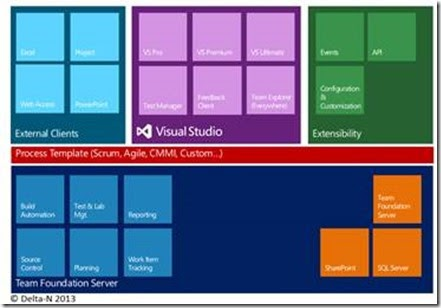
\includegraphics[scale=0.7]{./4.jpg}
		\end{center}
		\caption{نمای سطح بالای \lr{TFS}}
	\end{figure}

همان‌طور که در شکل شماره «۲» مشاهده ‌می‌شود (بدون پرداختن به هر جنبه به‌طور مستقل)، \lr{TFS} کاربردهای بسیار زیادی دارد و اساس بسیاری از موارد است. این اجازه را به ما می‌دهد تا منابع، مشکلات، برنامه‌ریزی و ساختن تست و... را به‌خوبی مدیریت کنیم. مهم‌ترین ویژگی \lr{TFS} توسعه‌پذیر \footnote{extensibility} آن است که آن را فوق‌العاده می‌کند؛ به این صورت که هر چیزی که وجود ندارد، یا می‌تواند ساخته شود و یا می‌تواند تغییر کند. این دقیقا همان چیزی است که استفاده از \lr{TFS} را برای سازمان‌ها مناسب می‌کند. ویژگی دیگر آن تنظیم‌پذیری \footnote{adjustability}و گستردگی آن است که هم می‌تواند تبدیل به نقطه قوت و هم نقطه ضعف آن شود؛ زیرا این ابزارها خاص منظوره هستند و عمل‌کرد آن‌ها باید بسته به کاربردشان  مقایسه و بررسی شود.


نحوه‌ی کار \lr{TFS} بدین صورت است که با \lr{process template}ها کار می‌کند. این قالب‌\footnote{template}ها از بخش‌های مختلفی شامل 
\begin{itemize}
	\item مورد کاری\footnote{\lr{work item}}
	\item گزارش‌ها
	\item مستندات
	\item نوع\footnote{type}‌ها
	\item و...
\end{itemize}
است و اجباری در انتخاب فرآیند انتخاب شده ندارد و دست مهندس نرم‌افزار را باز می‌گذارد.

\lr{TFS} می‌تواند در هر متدولوژی‌ای استفاده شود.  بسته به نوع متدولوژی‌ای که از آن استفاده می‌کنیم، مورد کاری تعریف می‌شود. این انعطاف‌پذیری زیاد باعث می‌شود که ساختار همه‌ی آن‌ها یکسان باشد.